%
% This is the LaTeX template file for lecture notes for EE 382C/EE 361C.
%
% To familiarize yourself with this template, the body contains
% some examples of its use.  Look them over.  Then you can
% run LaTeX on this file.  After you have LaTeXed this file then
% you can look over the result either by printing it out with
% dvips or using xdvi.
%
% This template is based on the template for Prof. Sinclair's CS 270.

\documentclass[twoside]{article}
\usepackage{graphics}
\usepackage{graphicx}
\setlength{\oddsidemargin}{0.25 in}
\setlength{\evensidemargin}{-0.25 in}
\setlength{\topmargin}{-0.6 in}
\setlength{\textwidth}{6.5 in}
\setlength{\textheight}{8.5 in}
\graphicspath{ {images/} }
\setlength{\headsep}{0.75 in}
\setlength{\parindent}{0 in}
\setlength{\parskip}{0.1 in}

%
% The following commands set up the lecnum (lecture number)
% counter and make various numbering schemes work relative
% to the lecture number.
%
\newcounter{lecnum}
\renewcommand{\thepage}{\thelecnum-\arabic{page}}
\renewcommand{\thesection}{\thelecnum.\arabic{section}}
\renewcommand{\theequation}{\thelecnum.\arabic{equation}}
\renewcommand{\thefigure}{\thelecnum.\arabic{figure}}
\renewcommand{\thetable}{\thelecnum.\arabic{table}}

%
% The following macro is used to generate the header.
%
\newcommand{\lecture}[4]{
   \pagestyle{myheadings}
   \thispagestyle{plain}
   \newpage
   \setcounter{lecnum}{#1}
   \setcounter{page}{1}
   \noindent
   \begin{center}
   \framebox{
      \vbox{\vspace{2mm}
    \hbox to 6.28in { {\bf EE 382C/361C: Multicore Computing
                        \hfill Fall 2016} }
       \vspace{4mm}
       \hbox to 6.28in { {\Large \hfill Lecture #1: #2  \hfill} }
       \vspace{2mm}
       \hbox to 6.28in { {\it Lecturer: #3 \hfill Scribe: #4} }
      \vspace{2mm}}
   }
   \end{center}
   \markboth{Lecture #1: #2}{Lecture #1: #2}
   %{\bf Disclaimer}: {\it These notes have not been subjected to the
   %usual scrutiny reserved for formal publications.  They may be distributed
   %outside this class only with the permission of the Instructor.}
   \vspace*{4mm}
}

%
% Convention for citations is authors' initials followed by the year.
% For example, to cite a paper by Leighton and Maggs you would type
% \cite{LM89}, and to cite a paper by Strassen you would type \cite{S69}.
% (To avoid bibliography problems, for now we redefine the \cite command.)
% Also commands that create a suitable format for the reference list.
\renewcommand{\cite}[1]{[#1]}
\def\beginrefs{\begin{list}%
        {[\arabic{equation}]}{\usecounter{equation}
         \setlength{\leftmargin}{2.0truecm}\setlength{\labelsep}{0.4truecm}%
         \setlength{\labelwidth}{1.6truecm}}}
\def\endrefs{\end{list}}
\def\bibentry#1{\item[\hbox{[#1]}]}

%Use this command for a figure; it puts a figure in wherever you want it.
%usage: \fig{NUMBER}{SPACE-IN-INCHES}{CAPTION}
\newcommand{\fig}[3]{
			\vspace{#2}
			\begin{center}
			Figure \thelecnum.#1:~#3
			\end{center}
	}
% Use these for theorems, lemmas, proofs, etc.
\newtheorem{theorem}{Theorem}[lecnum]
\newtheorem{lemma}[theorem]{Lemma}
\newtheorem{proposition}[theorem]{Proposition}
\newtheorem{claim}[theorem]{Claim}
\newtheorem{corollary}[theorem]{Corollary}
\newtheorem{definition}[theorem]{Definition}
\newenvironment{proof}{{\bf Proof:}}{\hfill\rule{2mm}{2mm}}

% **** IF YOU WANT TO DEFINE ADDITIONAL MACROS FOR YOURSELF, PUT THEM HERE:

\begin{document}
%FILL IN THE RIGHT INFO.
%\lecture{**LECTURE-NUMBER**}{**DATE**}{**LECTURER**}{**SCRIBE**}
\lecture{20}{November 3}{Vijay Garg}{Muhammad Raza Mahboob}
%\footnotetext{These notes are partially based on those of Nigel Mansell.}

% **** YOUR NOTES GO HERE:

% Some general latex examples and examples making use of the
% macros follow.  
%**** IN GENERAL, BE BRIEF. LONG SCRIBE NOTES, NO MATTER HOW WELL WRITTEN,
%**** ARE NEVER READ BY ANYBODY.

\section*{Agenda}
This lecture focused on Hashing and introduction of Transactional Memory. Major concepts discussed -:
\begin{itemize}
    \item Hashing basics
    \item Resizing Problem for Closed Addressing
    \item Chained Hashing
    \item Transactional Memory
\end{itemize} 

\section{Introduction}
Link list provides us with operations having O(n) complexity. In order to reduce the time complexity to constant time, we use Hashing. Hashing function is applied to the object and the result is an index (integer) and the item should be stored at that index in the bucket array. While Hashing we assume that the items are uniformly distributed so that each item most likely have a different hash value. Hashing comes in 2 different flavors: 
\begin{itemize}
\item Closed Addressing: Each item has a fixed bucket in the table and each bucket can contain several items in the form of a linked list.
\item Open Addressing: Each item could end up in a different bucket in the table and each bucket contains at most one item. 
\end{itemize}


\section{Resizing Problem}
Resizing is to allocate a new bigger bucket array and redistribute the existing items using the updated hash function which uses the new size. For closed addressing, we require resizing when the items in the individual buckets increases over a certain threshold which causes a linear search on the bucket list for the Hash operations. There are 2 different criteria for resizing:
\begin{itemize}
    \item Global threshold: When the size of X number of buckets increases over a certain threshold. (i.e X = 1/4)  
    \item Bucket threshold: When the size of any bucket increases over the threshold value.
\end{itemize} 
The new size of the bucket array is generally twice the original size in order to amortize the cost of copying the existing items in the new bucket array. 

There are 3 different techniques of resizing: coarse grained locking, fine grained locking and lock free resizing.
\subsection{Coarse Grained Locking}
The main idea of Coarse grained locking is very simple, there is one lock for the entire bucket array. Acquire that lock and start the resizing process which is to create a new bucket array and copy over all the existing elements in the new array using the updated hash function. 
Coarse grained lock resizing is very simple and easy to implement but it has the issue of sequential bottleneck. Only one thread can operate at any time which causes performance issues.



\subsection{Fine Grained Locking}
In fine grained lock resizing, there is a separate lock associated with each bucket which has to be acquired before performing any operation (i.e. insert) on that bucket. So while resizing, the first step is to acquire all the locks in ascending order and make sure that the table reference didn't change between the resize decision and the lock acquisition. After acquiring the locks, allocate the new super sized table and start transferring the existing elements into the new table. As shown in \ref{fig:1}, we take individual locks on each bucket, create a new bigger bucket array, copy over the existing elements and then map any new elements to the new array. 

\begin{figure}[h]
\centering
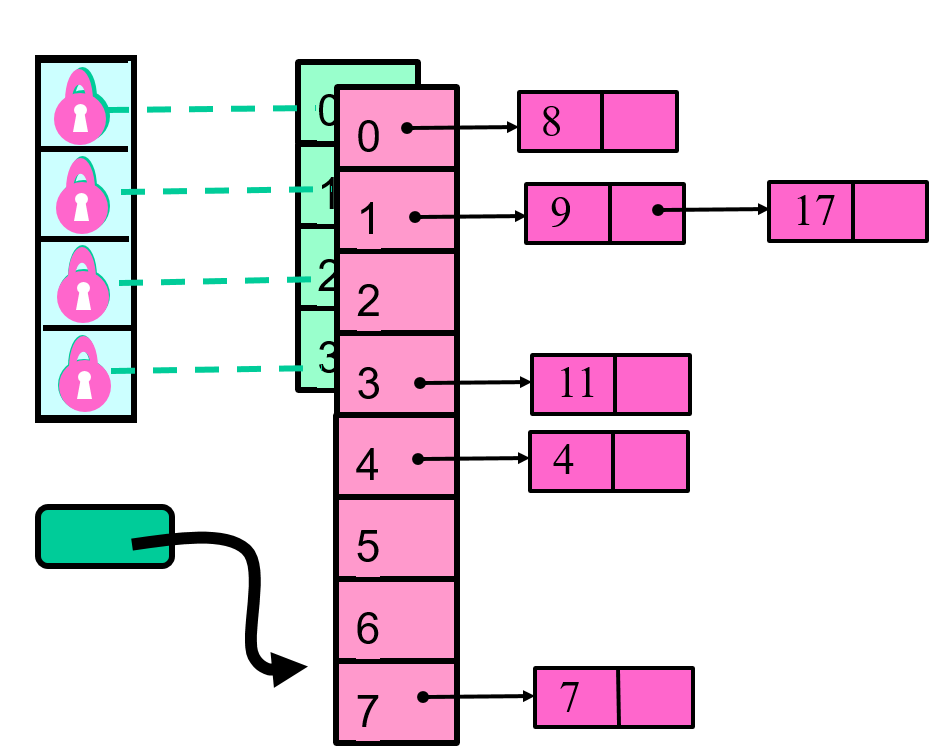
\includegraphics[scale=0.25]{Fine}
\caption{Fine Grained Locking}
\label{fig:1}
\end{figure}

\emph{Striped Locks:} Instead of allocating new locks for the new array, we use the existing locks. Since the size of the new array is double the size of original array, we use the each existing lock to cover one more bucket in the new array based on the symmetry.  

\emph{Read Locks:} We leverage the insight that most common operations is search on the hash table and so we keep 2 different kinds of locks: read lock and write lock. So multiple threads can take the read lock and start searching on the hash bucket.

\subsection{Lock Free Resizing}
The idea of resizing is to remove the existing element and put it at a new location in the new array. These are 2 different operations but CAS(CompareAndSwap) only allows us to do one operation so we either need a double-compare-and-swap operation or a new idea for lock free resizing. The idea is to keep the items fixed in an ordered linked list and move the buckets. All the items are reachable from the top bucket but the additional buckets are shortcuts that allow us to achieve constant time retrieval.\\
We keep all the elements in a linked list with special order. The order will enable us to easily point new buckets in the linked list. We use the Recursive Split Ordering meaning that we recursively divide the existing bucket into two based on the least significant bit of the item. The ordering is based on the least significant bits. Starting from the least significant bit, start ordering and until all the elements are ordered. An example is given in \ref{fig:2} where each element is first sorted on the least significant bit and then on the second last significant bit. So if you have, two keys: a and b, a precedes b if and only if the bit reversed (least significant i bits) value of a is smaller than the bit reversed value of b as shown in \ref{fig:3}. 
\begin{figure}[h]
\centering
\includegraphics[scale=0.25]{ordering}
\caption{Special Ordering of items}
\label{fig:2}
\end{figure}

\begin{figure}[h]
\centering
\includegraphics[scale=0.25]{mapping}
\caption{Reverse Ordering}
\label{fig:3}
\end{figure}


Each bucket is mapped according to the reverse order of the bits of the first element in the linked list found by traversing from an existing bucket. But this causes an issue when removing a node having both the bucket pointer and the previous node pointer in the linked list using a single CAS operation. In order to cater for this problem, we use Sentinel Node for each bucket and initialize them whenever we need to point a bucket. So first create the Sentinel node and point it to the real node in the list. After that adjust the previous pointer to point to this sentinel node and finally add the bucket pointer to the sentinel.  

\section{Closed Hashing}

\subsection{Linear Probing}
In open addressing we keep the bucket array which hold the actual items instead of pointing to a new list. Whenever an item x needs to added, we apply the hash function on the item and try to put the item at H(x) index. If that index is already occupied then we move forward from that index until we find an empty spot to allocate x. For the Contain(x) operation, we start from H(x) and then search linearly until we find x or there is an empty bucket.\\
\textbf{Advantages:}
\begin{itemize}
\item Good Locality which means less Cache misses 
\end{itemize}
\textbf{Disadvantages:}
\begin{itemize}
\item As the number of total items ratio to bucket size increases (M/N) more cache misses because we maybe searching in several unrelated buckets
\item Clustering effect of keys into neighboring buckets 
\end{itemize}

\subsection{Cuckoo Hashing}
Cuckoo hashing leverages the \textbf{power of 2} concept and creates 2 bucket arrays instead of one and keep two different hash functions, one for each array. For Insert(x) operation, we take the H1(x) and look at the resulting index in first array. If it's empty then just place x there else if there is an element y at H1(x) then take H2(x) and look at the resulting position in the second array. If it is empty then place x there else evict y, place x at H1(x) and recursively insert y at H2(y) and so on. The same idea is used for searching purposes.\\
\textbf{Advantages:}
\begin{itemize}
\item No clustering issue
\end{itemize}
\textbf{Disadvantages:}
\begin{itemize}
\item 2 tables
\item The hash functions could be complex
\item As M/N increases, the relocation cycle increases
\end{itemize}   

\subsection{Hopscotch Hashing}
In Hopscotch hashing we have a single array and a simple hash function but we define neighborhood of original bucket. While adding an item, probe linearly to find an open slot and move the empty slot via sequence of displacements into the hop-range of H(x). For Contain(x) operation, search in at most H buckets (the hop range) based on the hop-info bitmap. \\
\textbf{Advantages:}
\begin{itemize}
\item Good locality and cache behavior
\item Good performance as table density increases
\item Optimize the common operation (Contains) at the expense of Insert
\end{itemize}
\textbf{Disadvantages:}
\begin{itemize}
\item Does not work well in all scenarios like Cuckoo Hashing
\end{itemize}   
 
\section{Trasactional Memory}
Unitl now we have seen 2 different mechanisms to achieve mutual exclusion i.e. Lock based and lock free. Transactional memory is another concept used in this regard. \\
\begin{figure}[h]
\centering
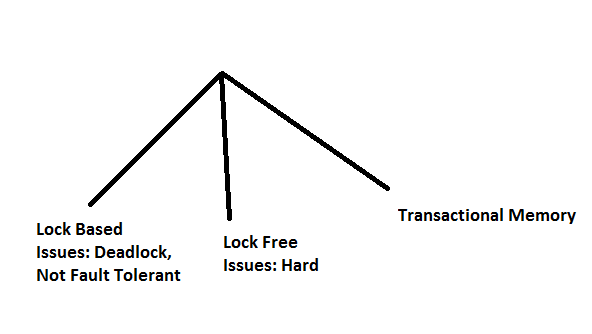
\includegraphics[scale=0.5]{illus}
\caption{Different Concepts for Mutual Exclusion}
\label{fig:4}
\end{figure}

The concept of Transactional memory is derived from Databases where we have similar issues like Concurrency and Failures. Jim Gray pioneered the concept of transactions for databases. The main construct of a Transaction is that we have \textit{begin.transaction} at the start followed by several reads, writes and abort operations and then finally \textit{end.transaction} which is also called commit transaction.  
Transactions in databases provide 4 guarantees which are commonly known as ACID:
\begin{itemize}
\item Atomicity : All or nothing
\item Consistency : transaction will bring the database from one valid state to another
\item Isolation  : concurrent execution of transactions results in a system state that would be obtained if transactions were executed serially
\item Durability : persistence even in the events of power loss or error
\end{itemize}

\section*{References}
\beginrefs
\bibentry{1}{\sc Vijay K Garg},
Introduction to Multicore Computing
\bibentry{2}{\sc Maurice Herlihy, Nir Shavit}, Hashing and Natural Parallism, Companion slides for
The Art of Multiprocessor Programming
\endrefs


\end{document}





